\documentclass{scrartcl} 
\usepackage[ngerman]{babel}
\usepackage[utf8]{inputenc}
\usepackage[T1]{fontenc}
\usepackage{lmodern}
%\usepackage{titletoc}
\usepackage{enumerate}
\usepackage{graphicx}
%\usepackage{a4wide}
\usepackage{float} % lädt das Paket zur Verwendung von zusätzlichen Positionsbefehlen
% volle Seite nutzen
\usepackage{fullpage} 
\usepackage{lastpage}
\usepackage{amssymb, amstext, amsmath}
\usepackage{mathtools}
\usepackage{enumitem}
\usepackage{float}
\usepackage{gauss}
\usepackage{graphicx}
\usepackage{hyperref}
\usepackage{titleref}

\usepackage[framemethod=tikz]{mdframed}

% Shorthands
\newcommand*\iffdef{\overset{\text{def}}{\iff}}
\DeclarePairedDelimiter\abs{\lvert}{\rvert}
\DeclarePairedDelimiter\norm{\lVert}{\rVert}

% https://www.google.de/design/spec/style/color.html#color-color-palette
\definecolor{colorBackground}{HTML}{BDBDBD} % Grey 400
\definecolor{colorDefinition}{HTML}{4CAF50} % Green 500
\definecolor{colorNotiz}{HTML}{81D4FA}      % Light Blue 200
\definecolor{colorWarnung}{HTML}{FF9800}    % Orange 500
\definecolor{colorBeispiel}{HTML}{0288D1}   % Light Blue 700
\definecolor{colorSatz}{HTML}{009688}       % Teal 500

\mdfdefinestyle{box}{
	topline=false,
	bottomline=false,
	rightline=false,
	linewidth=4pt,
    backgroundcolor=none,
    apptotikzsetting={\tikzset{mdfbackground/.append style={fill=colorBackground,fill opacity=.4}}},
    frametitlefont=\sffamily\bfseries\color{black},
    splittopskip=.5cm,
    frametitlebelowskip=.3cm,
}

% Definition
\mdtheorem[
  style=box,
  linecolor=colorDefinition,
]{Def}{Defintion}[section]

% Notiz
\mdtheorem[
  style=box,
  linecolor=colorNotiz,
]{Notiz}{Notiz}[section]

% Warnung
\mdtheorem[
  style=box,
  linecolor=colorWarnung,
]{Warnung}{Warnung}[section]

% Beispiel
\mdtheorem[
  style=box,
  linecolor=colorBeispiel,
]{Beispiel}{Beispiel}[section]

% Satz
\mdtheorem[
  style=box,
  linecolor=colorSatz,
]{Satz}{Satz}[section]


\hypersetup{
    hidelinks,
    colorlinks=false,
    linktoc=all
}

\makeatletter
  \edef\g@post{\relax$}

% Begin gauss vline fix$
% patch gauss macros for doing their work in `align'
% and other amsmath environments; see
% http://tex.stackexchange.com/questions/146532/
\usepackage{etoolbox}
\makeatletter
\patchcmd\g@matrix
 {\vbox\bgroup}
 {\vbox\bgroup\normalbaselines}% restore the standard baselineskip
 {}{}
\makeatother
\newcommand{\BAR}{%
  \hspace{-\arraycolsep}%
  \strut\vrule % the `\vrule` is as high and deep as a strut
  \hspace{-\arraycolsep}%
}
% End gauss vline fix

\usepackage{fancyhdr}

\newcommand{\fett}[1]{\textbf{#1}}
\newcommand{\kursiv}[1]{\textit{#1}}
\newcommand{\unterstrichen}[1]{\underline{#1}}
\newcommand{\vereinigung}{\cup}
\newcommand{\schnitt}{\cap}
\newcommand{\logischund}{\wedge}
\newcommand{\logischoder}{\vee}
\newcommand{\natuerlichezahlen}{\mathbb{N}}
\newcommand{\binaerezahlen}{\mathbb{B}}
\newcommand*\dashline{\hspace{-0.6em}\rotatebox[origin=c]{90}{\scalebox{-0.5}[1]{$-~~-$}}\hspace{-0.6em}}

\newcommand{\linkTo}[1]{\hyperref[#1]{\underline{#1}}}
\newcommand{\linkToRef}[2][ref]{\hyperref[#1]{\underline{#2}}}

\def\Uebung{MA 0901, Lineare Algebra\\Zusammenfassung}

%Anfang == Zusammensetzen des Titels
\title{\Uebung}
%Ende == Zusammensetzten des Titels


\author{Felix Beil \\
Maximilian Gießelmann \\
Simon Huber \\
Sebastian Kneuer \\
Mit freundlicher Unterstützung durch Simon Plazotta\\
TUM SS 2015}

%%%%%%%%%%%%%%%%%%%%%%%%%%%%%%%%%%%%%%%%%%%%%%%%%%%%%%%%%%%%%%%%%%%%%%%%%%%%%%%%%%%%%%%%%%%%%%%%%%%%%%%%%
% Auto Recompile in ShareLatex:                                                                         %
% var recompileInterval=setInterval(function(){$('a[ng-click="recompile()"]').trigger('click')},40000); %
%                                                                                                       %
% Stop Auto Recompile:                                                                                  %
% clearInterval(recompileInterval);                                                                     %
%%%%%%%%%%%%%%%%%%%%%%%%%%%%%%%%%%%%%%%%%%%%%%%%%%%%%%%%%%%%%%%%%%%%%%%%%%%%%%%%%%%%%%%%%%%%%%%%%%%%%%%%%

\headsep1em
\parindent0em
\headheight13.87178pt

\graphicspath{{images/}}

\begin{document}
\pagestyle{fancy}
\lhead{}
\chead{\leftmark}
\rhead{\hyperref[top]{\thepage} von \pageref{LastPage}}
\cfoot{}
\maketitle
% \vspace{5cm}
\label{top}
\tableofcontents

\newpage
\section{Matrizen}
\label{Matrix}
\subsection{Definitionen / Begriffserklärungen}

\begin{itemize}
\item Eine \textbf{Matrix}:
\[A = 
\begin{pmatrix} 
a_{1,1} & a_{1,2} & \dots  & a_{1,n}\\
a_{2,1} & a_{2,2} & \dots  & a_{2,n}\\
\vdots & \vdots &  &\vdots \\
a_{m,1} & a_{m,2} & \dots  & a_{m,n}
\end{pmatrix}\]

\item $a_{1,1}$ heißt \label{Eintrag} \textbf{Eintrag}

\item Eine 1 x n-Matrix $(a_{1}, \dots, a_n) \in K^{1xn} $ heißt \label{Zeilenvektor}\textbf{Zeilenvektor}

\item Eine $mx1$-Matrix $\begin{pmatrix} a_1\\ \vdots \\ a_m \end{pmatrix} \in K^{mx1} $ heißt \label{Spaltenvektor}\textbf{Spaltenvektor}

\item $K^m := K^{mx1} $ m-\label{Standardraum}\textbf{dimensionalen Standardraum}

\item Eine Matrix $A \in K^{mxn} $ mit $m=n$ heißt \label{quadratische Matrix}\textbf{quadratische \linkTo{Matrix}}

\item \label{transponierte Matrix} \textbf{transponierte \linkTo{Matrix}}: 
\[
\begin{pmatrix}
1 & 2 & 3\\
4 & 5 & 6
\end{pmatrix}^T =
\begin{pmatrix}
1 & 4 \\
2 & 5\\
3 & 6
\end{pmatrix}
\]


\item Eine \linkTo{quadratische Matrix} heißt \label{symmetrische Matrix} \textbf{symmetrische \linkTo{Matrix}}, falls $A^T = A$ gilt.

\item \label{Transistions-Matrix} \textbf{Transistions-\linkTo{Matrix}} (am Beispiel der Google-Matrix)\\
Durch Anzahl Links zu Seite geteilt Durch alle Seiten ergibt den Wert in der W-Matrix. Dadurch kann man dann die Wahrscheinlichkeit berechnen, dass ein Zufallssurfer auf die Seite trifft.

\item \label{matrix Multiplikation} \textbf{\linkToRef[Matrix]{matrix} Multiplikation}:\\
Nur möglich, wenn $A_{m,\textbf{n}}$ und $B_{\textbf{n},o}$! Dimmension der neuen Matrix ergibt sich aus der Zeilen Anzahl der ersten Matrix und der Spalten Anzahl der zweiten Matrix $\Rightarrow C_{m,o}$
\begin{figure}[htp]
    \centering
    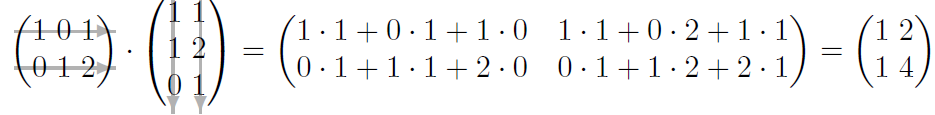
\includegraphics[width=15cm]{Multi}
%    \caption{\linkToRef[Matrix]{matrix} Multiplikation}
    \label{fig:multiplikation}
\end{figure}

\end{itemize}

\subsection{Regeln}

\begin{Satz} 
Für Matrizen gelten die folgenden Regeln.
\begin{enumerate}[label={(\alph*)}]
\item $(K^{m \times n}, +)$ ist eine abelsche Gruppe.
\item Für alle $A,B \in K^{m \times n}$ und $s,s' \in K$ gelten:
    \begin{enumerate}[label={(\arabic*)}]
    \item $s \cdot (A + B) = s \cdot A + s \cdot B$,
    \item $(s + s') \cdot A + s' \cdot A$,
    \item $s \cdot (s' \cdot A) = (ss') \cdot A$,
    \item $1 \cdot A = A$.
    \end{enumerate}
\item Seien $A,B,C$ Matrizen, so dass jeweils die unten gebildeten Summen und Produkte definiert sind. Dann gelten:
    \begin{enumerate}[label={(\arabic*)}]
    \item $(A \cdot B) \cdot C = A \cdot (B \cdot C)$,
    \item $A \cdot (B + C) = A \cdot B + A \cdot C$,
    \item $(A + B) \cdot C = A \cdot C + B \cdot C$.
    \item Für
        \begin{align*}
        I_n := \begin{pmatrix}
            1 & 0 & & \dots & 0 \\
            0 & 1 & & & \vdots \\
            & & \ddots & & \\
            \vdots & & & 1 & 0 \\
            0 & \dots & & 0 & 1
        \end{pmatrix} \in K^{n \times n}
        \end{align*}
        (die \textbf{Einheitsmatrix}) gelten $I_n \cdot A = A$ und $B \cdot I_n = B$.
    \end{enumerate}
\end{enumerate}
\begin{itemize}
\item $A \cdot B = B \cdot A $ ist FALSCH
\item $(AB)^T = B^T \cdot A^T$
\end{itemize}
\end{Satz}

\newpage
\section{Lineare Gleichungssysteme}
\label{Lineares Gleichungssystem}
\subsection{Definitionen / Begriffserklärungen}

\begin{itemize}
\item Kurz: \textbf{LGS}
\item \label{Lösungsmenge}\textbf{Lösungsmenge} ist die Menge aller $x \in K^n $, die die Gleichung erfüllen.
\item Gleichung: $A \cdot x = b$ mit $A \in \mathbb{K}^{m \times n}$ und $b \in \mathbb{K}^m$ 
\item Das \linkTo{LGS} heißt \label{homogenes LGS} \textbf{homogen}, falls $b = \begin{pmatrix} 0\\ \vdots \\ 0\end{pmatrix}$, sonst \label{inhomogens LGS} \textbf{inhomogen}.
\end{itemize}

\subsection{Koeffizentenmatrix}
\label{Koeffizentenmatrix} 

\begin{align*}
x_1 + 2x_3 + x_4 &= -3\\
2x_1 + 4x_3 - 2x_4 &= 2\\
x_2 -x_4 &= 2 \\
x_1 + 2x_3 + 2x_4 &= -5
\end{align*}
\[
\Rightarrow A = 
\begin{pmatrix}
1 & 0 & 2 & 1\\
2 & 0 & 4 & -2\\
0 & 1 & 0 & -1\\
1 & 0 & 2 & 2 
\end{pmatrix}, b = \begin{pmatrix}
-3 \\
2 \\
2\\
-5
\end{pmatrix}
\]

\subsection{Erweiterte Koeffizentenmatrix}
\label{erweiterete Koeffizentenmatrix} 

\[
\Rightarrow A = 
\left(\begin{array}{cccc|c}
1 & 0 & 2 & 1 & -3 \\
2 & 0 & 4 & -2 & 2\\
0 & 1 & 0 & -1 & 2\\
1 & 0 & 2 & 2 & -5
\end{array}\right)
\]

\subsection{Elementare Zeilenoperationen}
\label{elementare Zeilenoperationen}

\begin{itemize}
\item \textbf{Typ I:} Vertauschen zweier Zeilen
\item \textbf{Typ II:} Multiplizeieren einer Zeile mit einem Skalar $s \in K \setminus \{0\}$
\item \textbf{Typ III:} Addieren des s-fachen einer Zeile zu einer anderen, wobei $s \in K$
\end{itemize}

\subsection{Zeilenstufenform}
\label{Zeilenstufenform}

\begin{Def}
Es sei $A \in K^{m \times n}$. Wir sagen, dass $A$ in \textbf{Zeilenstufenform} ist, falls gelten:
\begin{enumerate}[label={(\alph*)}]
\item Beginnt eine Zeile mit $k$ Nullen, so stehen unter diesen Nullen lauter weitere Nullen.
\item Unter dem ersten Eintrag $\neq 0$ eine jeden Zeile (falls diese nicht nur aus Nullen besteht) stehen lauter Nullen.
\end{enumerate}
Wir sagen, dass $A$  in \textbf{strenger Zeilenstufenform} ist, falls zusätzlich gilt:
\begin{enumerate}[label={(\alph*)}]
\setcounter{enumi}{2}
\item Über dem ersten Eintrag $\neq 0$ einer jeden Zeile (falls diese nicht nur aus Nullen besteht) stehen lauter Nullen.
\end{enumerate}
\end{Def}

\begin{Beispiel} 
Zur Illustration mögen folgende Beispiele dienen:
\begin{enumerate}[label={(\arabic*)}]
\item Die Matrix $\begin{pmatrix} 0 & 1 & 2 \\ 1 & 0 & 0 \\ 0 & 0 & 0 \end{pmatrix}$ ist \textit{nicht} in Zeilenstufenform.
\item Die Matrix $\begin{pmatrix} 0 & 1 & 2 \\ 0 & 1 & 1 \\ 0 & 0 & 0 \end{pmatrix}$ ist \textit{nicht} in Zeilenstufenform.
\item Die Matrix $\begin{pmatrix} 1 & 2 & -1 \\ 0 & 0 & -1 \\ 0 & 0 & 0 \end{pmatrix}$ ist in Zeilenstufenform, aber nicht in Strenger Zeilenstufenform.
\item Die Matrix $\begin{pmatrix} 1 & 2 & 0 \\ 0 & 0 & -1 \\ 0 & 0 & 0 \end{pmatrix}$ ist in strenger Zeilenstufenform.
\end{enumerate}
\end{Beispiel}

\subsection{Gauß-Algorithmus}
\label{Gauss}

\begin{tabular}{p{0.13\textwidth}p{0.85\textwidth}}
\textbf{Eingabe:} & Eine Matrix $A \in K^{m \times n}$. \\
\textbf{Ausgabe:} & Eine Matrix $B \in K^{m \times n}$ in (strenger) Zeilenstufenform, die aus $A$ durch elementare Zeilenoperationen hervorgeht.
\end{tabular}

\begin{enumerate}[label={(\arabic*)}]
\item Setze $B := A$.
\item $B$ sei bis zur $r$-ten Spalte in Zeilenstufenform, d.h. (a) und (b) aus der Definition seien bis zur $r$-ten Zeile erfüllt. (Hierbei ist $r = 0$ möglich!)
\item Falls $r = m$, so ist $B$ in Zeilenstufenform. Falls streneg Zeilenstufenform gewünscht ist, gehe zu (8).
\item Suche den am weitesten links stehenden Eintrag $\neq 0$ von $B$ unterhalb der $r$-ten Zeile. (Falls es mehrere solche Einträge gibt, wähle einen aus.)
\item Bringe diesen Eintrag in die $(r + 1)$-te Zeile (Operation Typ I).
\item Erzeuge unterhalb dieses Eintrags lauter Nullen (Operation Typ III, optional auch II).
\item Gehe zu (2).
\item Bringe $B$ auf strenge Zeilenstufenform (Operation Typ III).
\end{enumerate}

\subsection{Rang}
\label{Rang}

\begin{Def}
Der \textbf{Rang} von A ist die Anzahl $r$ Zeilen in $A'$, die mindestens einen \linkTo{Eintrag} $\neq 0$ haben. $A'$ ist die \linkTo{Zeilenstufenform} von $A$. Es muss keine strenge \linkTo{Zeilenstufenform} vorliegen.
\[r := rg(A)\]
\end{Def}
\begin{Beispiel}
\begin{align*}
    A &= \begin{pmatrix}
        1 & 8 & 2 & 0 \\
        0 & 0 & 1 & 2 \\
        0 & 0 & 0 & 0 \\
    \end{pmatrix}\\
    rg(A) &= 2
\end{align*}
\end{Beispiel}


\subsection{Lösbarkeit}
\label{Lösbarkeit}
Lösbarkeits-Fälle:
	\begin{itemize}
		\item $b_{r+1} \neq 0 \rightarrow $ keine Lösung
		\item $b_{r+1} = 0 \rightarrow $ LSG lösbar. Unterfälle:
		\begin{itemize}
			\item $ n = r \rightarrow $ eindeutige Lösung
			\item $n > r \rightarrow $ keine eindeutige Lösung, $n - r = \# $ freier Variablen
		\end{itemize}
	\end{itemize}
	
\begin{Beispiel}
\begin{itemize}
\item 
$
\begin{pmatrix}
	1 & 0 & 2 \\ 
	0 & 1 & 7
\end{pmatrix}
	\rightarrow r = 2 = n \rightarrow
$ LSG lösbar

\item 
$
\begin{pmatrix}
	1 & 2 & 1 \\ 
	0 & 0 & 0 \\ 
	0 & 0 & 0
\end{pmatrix}  $\\
$ r = 1 \neq 2 = n \\\qquad b_{r+1} = b_2 = 0 \rightarrow $ LSG ist lösbar, $n - r = 1 $ freie Variablen => Lösung nicht eindeutig.

\item
\[
\left(\begin{array}{ccc|c}
	1 & 2 & 3 & 4 \\ 
	0 & 0 & 0 & 2
\end{array}\right)  \]
$ r = 1 \qquad b_{r+1} = b_2 = 2 \neq 0 \Rightarrow $ LSG nicht lösbar.

\end{itemize}
\end{Beispiel}

Rangkriterien für Lösbarkeit von LGS:
\begin{itemize}
	\item $A \in K^{mxn} $ Koeff. Matrix (m Glg., n Unbekannte)
	\item $b \in K^{mxn} $ rechte Seite
	\item $rg(A|B) \in \{rg(A), rg(A) + 1\} $ (einzigen Beiden Möglichkeiten)
	und es gilt:
	\begin{itemize}
	\item LGS lösbar $\Leftrightarrow rg(A|B) = rg(A)$
	\item In diesem Fall: Lösung Eindeutig $\leftrightarrow rg(A) = rg(A|B) = n$
	\item Lösung nicht Eindeutig $\leftrightarrow rg(A) < n$ (und $n-rg(A) = \# $ freier Variablen)
	\end{itemize}
\end{itemize}

\newpage
\section{Vektorräume}
\label{Vektorraum}

\subsection{Unterraum}
\label{Untervektorraum}

\begin{Def}

Sei $V$ ein $K$-Vektorraum. Eine Teilmenge $U \subseteq V$ heißt ein \textbf{Unterraum} (auch: Untervektorraum, Teilraum), falls gelten:
\begin{enumerate}[label={(\arabic*)}]
\item $U \neq \emptyset$
\item Für $v,w \in U$ ist auch $v + w \in U$ (also ist $(U, +)$ eine Untergruppe)
\item Für $a \in K$ und $v \in U$ gilt $a \cdot v \in U$
\end{enumerate}
Aus der Definition folgt sofort:
\begin{itemize}
\item Jeder Unterraum enthält den Nullvektor
\item Mit den Operationen ``$+$'' und ``$\cdot$'' von $V$ wird ein Unterraum $U$ selbst ein $K$-Vektorraum
\end{itemize}
\end{Def}
\begin{Notiz}
Der \label{Spann} Spann ist der kleinste Untervektorraum, der die Menge A enthält.
\end{Notiz}

\subsubsection{Untervektorräume}
\begin{Def}
	$V~K-VR$ (K körper) $(V,+,\cdot)$ \\
	$U \subseteq V$ heißt Unter(vektor)raum $\Leftrightarrow$
	\begin{enumerate}[label={(\arabic*)}]
		\item % (1)
		$U \neq \oslash$
		
		\item % (2)
		$\forall v,w \in U \Rightarrow v + w \in U$ 
		
		\item % (3)
		$\forall a \in K, v \in U \Rightarrow a \cdot v \in U$
	\end{enumerate}


	Jeder Untervektorraum  enthält die 0 (Prop 3.3a) $0 \cdot v = 0 \in U$) Falls als eine Menge $U \leq V$ die 0 enthält, kann kein UVR sein.\\
	Schnitt von UVR ($U_1, U_2 \subseteq V$):
	\begin{enumerate}
	\item $U_1 \schnitt U_2 \subseteq V$ ist ein Unterraum.
	\item $U_1 + U_2 := \{u_1 + u_2 | u_1 \in U_1, u_2 \in U_2\}$ ist ein Unterraum.
	\item Ist $M \neq \emptyset$ eine nicht-leere Menge, deren Elemente Unterräume von $V$ sind, so ist auch der Schnitt ein Unterraum.
	\end{enumerate}
\end{Def}
	

\newpage
\section{Linearkombinationen}
\begin{Def}
    \begin{enumerate}[label={(\alph*)}]
    \item Es seien $v_1, ..., v_n \in V$ Vektoren. Ein Vektor $v \in V$ heißt \textbf{Linearkombination} von $v_1, ..., v_n$, falls es Skalare $a_1, ..., a_n \in K$ gibt mit
        \begin{align*}
            v = a_1v_1 + ... + a_nv_n
        \end{align*}
    \item Sei $S \subseteq V$ eine Teilmenge. Ein Vektor $v \in V$ heißt \textbf{Linearkombination} von $S$, falls es $n \in \mathbb{N}$ und $v_1, ..., v_n \in S$ gibt, sodass $v$ eine Linearkombination von $v_1, ..., v_n$ ist. Falls $S = \emptyset$, so ist der Nullvektor $0$ (die einzige) Linearkombination von $S$. ($0$ wird als leere Summe aufgefasst)
    \end{enumerate}
\end{Def}
\begin{Notiz}
    Eine Linearkombination ist ein Vektor, der die Koeffizienten für die einzelnen Variablen (Spalten in einer Matrix) von einem \linkToRef[Lineares Gleichungssystem]{Linearem Gleichungssystem} angibt.
\end{Notiz}

\subsection{Berechnung}
Siehe Rezept \ref{Linearkombination}.

\newpage
\section{Basen}
\label{Basis}

\begin{Def}
Eine Basis ist eine Teilmenge eines Vektorraumes, mit deren Hilfe sich jeder Vektor des Raumes eindeutig als endliche Linearkombination darstellen lässt. 


Eine Basis ist eine Menge von Vektoren aus den sich alle anderen Vektoren des Körpers ableiten lassen, indem Koeffizenten vor die Vektoren der Basis gesetzt werden.
\end{Def}
\begin{Beispiel}
\begin{align*}
v_1 := \begin{pmatrix} 1 \\ 0 \\ 1\\ 0 \end{pmatrix}, ~~~ v_2:= \begin{pmatrix} 0 \\ 1 \\ 0\\ 1 \end{pmatrix}, ~~~ v_3:= \begin{pmatrix} 1 \\ -1 \\ 2\\ 1 \end{pmatrix}, ~~~ v_4:= \begin{pmatrix} -1 \\ 0 \\ 2\\ 0 \end{pmatrix}
\end{align*}
Basis $B = \{v_1, v_2, v_3, v_4\}$ von $\mathbb{R}^4$
\end{Beispiel}

\begin{Beispiel}[Sehr einfaches Beispiel]
$B = \{(1)\}$ von $\mathbb{R}$


Man kann nun mit einem Koeffizenten x alle Zahlen $z \in \mathbb{R}$ bilden:\\
$z = x \cdot (1)$
\end{Beispiel}

\subsection{Erzeugendensystem}
\label{Erzeugendensystem}

Eine Basis ist also immer auch ein Erzeugendensystem, ein Erzeugendensystem ist genau dann eine Basis, wenn seine Vektoren linear unabhängig sind.

\newpage
\section{Lineare Codes}

Code $c \in \mathbb{F}_2^n$ ist ein Code aus dem Raum $\mathbb{F}_2 = \{0,1\}$ mit $n$ Stellen

\begin{Def}[Codewort]
Ein Codewort $c \in C$ besteht aus einem Informationswort und der Redundanz. Es wird durch eine (häufig rauschende) Leitung zum Empfänger gesendet.
\end{Def}

\begin{Def}[Informationswort]
Das Informationswort ist der Teil des Codeworts, dass die zu sendenden / empfangenen Informationen enthält.
\end{Def}
\begin{Def}[Redundanz]
Die Redundanz ist der Teil des Codeworts, der benutzt wird, um das Informationswort zu verifizieren und ggf. zu verbessern.
\end{Def}

\subsection{Generatormatrix}
\begin{Def}
Die Generatormatrix $G$ wird benutzt um aus dem Informationswort $x$ das Codewort $c$ zu berechnen.
\[
\begin{pmatrix} c_1 \\ \vdots \\ c_n \end{pmatrix} = G \cdot \begin{pmatrix} x_1 \\ \vdots \\ x_k \end{pmatrix}
\]
\end{Def}
\begin{Def}[Aufbau der Generatormatrix]
Beliebig.
\begin{Beispiel}
\[
G = \begin{pmatrix} I_K \\ A \end{pmatrix}
\]
\end{Beispiel}
\end{Def}

\subsection{Parity-Check-Matrix}
\begin{Def}
Die Parity-Check-Matrix wird benutzt um ein empfangenes Codewort $c$ zu verifizieren. Ist das empfangene Wort $c \in C$ (also gab es keine Fehler), so folgt daraus:
\[
P \cdot c = 0
\]
\end{Def}
\begin{Satz}[Aufbau der Parity-Check-Matrix, wenn G wie in Beispiel 6.1 aufgebaut ist]
\[
P = \begin{pmatrix} -A & I_{n-k} \end{pmatrix} \in K^{(n-k) \times n}
\]
\end{Satz}

\subsection{Hamming-Gewicht}

\begin{Def}
Das Hamming-Gewicht ist definiert durch
\[
w(c) := \Big| \Big\{ i \in \{ 1,...,n \} \Big| c_i \neq 0 \Big\} \Big|
\]
Das Hamming Gewicht gibt nur die Anzahl der Nichtnull Einträge an.
\end{Def}

\subsection{Hamming-Abstand}
\begin{Def}
Der Hamming-Abstand von zwei möglichen Codewörten ist definiert durch
\begin{align*}
d(c,c') := w(c - c') = \Big| \Big\{ i \in \{ 1, ..., n \} \Big| c_i \neq c'_i \Big\}\Big|
\end{align*}
und gibt die Anzahl der unterschidelichen Stellen in den Codewörten an.\\
Für den Code $C$ ist der Hamming-Abstand definiert durch
\begin{align*}
d(C) := min\Big\{ d(c, c') \Big| c, c' \in C, c \neq c' \Big\} = min w(c), c \in C \setminus \{0\}
\end{align*}
\end{Def}

\begin{Beispiel}
Das bedeutet: Sei ein (5,2)-Code gegeben und es gibt genau die 4 Codewörter $(0,0,0,0,0) $ $ (1,0,1,0,1) $ $ (0,1,0,1,1) $ $(1,1,1,1,0)$. Dann ist sein Minimalabstand 3, da mindestens 3 Elemente aus einem Codewort verändert werden müssen, um auf ein beliebiges anderes Codewort zu kommen.
\end{Beispiel}

\subsection{Variablen}
\begin{tabular}{ll}
$n$ & Dimension des Codewortes $c \in C$ \\
$k$ & Dimension des Informationswortes \\
$d$ & Informationsrate $ = \frac{k}{n}$
\end{tabular}

\begin{Warnung}
$d$ ist leicht zu verwechseln mit der Funktion $d(c, c') $ des Hamming-Abstands!
\end{Warnung}

\newpage
\section{Lineare Abbildungen}

\subsection{Kern}
\begin{Def}
Sei $\varphi: V \rightarrow W$ linear
\begin{align*}
    Kern(\varphi) := \{v \in V | \varphi(v) = 0\} \subseteq V
\end{align*}
\end{Def}
\begin{Notiz}
Der Kern ist die Menge an Werten, die in die Abbildung eingesetzt werden muss, damit $0$ raus kommt, vgl. \textbf{Nullstellen} von Funktionen
\end{Notiz}

\begin{Notiz}
$rg(A) = dim(Kern(A))$
\end{Notiz}

\subsection{Bild}
\begin{Def}
Sei $\varphi: V \rightarrow W$ linear
\begin{align*}
    Bild(\varphi) := \varphi(V) = \{\varphi(v) | v \in V \} \subseteq W
\end{align*}
\end{Def}
\begin{Notiz}
Das Bild gibt die Menge der Werte an, die durch die Abbildung erreicht werden können, vgl. \textbf{Wertebereich} von Funktionen
\end{Notiz}

\newpage
\section{Darstellungsmatrizen}
\label{Darstellungsmatrix}

\begin{Def}

$D_B(\varphi) \in \mathbb{K}^{n \times n} $ beschreibt $\varphi$ bezüglich $B$.

\end{Def}

\begin{Notiz}
  Spalten der Darstellungsmatrix $\Leftrightarrow$ Bilder der Basisvektoren
\end{Notiz}

\newpage
\section{Determinanten}
    \subsection{Signum / Vorzeichen}
        \begin{itemize}
            \item $S_n = := \{\sigma   :\{1, \dots, n\} \rightarrow \{1, \dots, n\} | \sigma~ist~bijektiv\}$
            \item $S_n$ heißen Permutationen.
            \item $sgn(\sigma) := (-1)^{w(\sigma)} $, das Vorzeichen / Signum von $\sigma$
        \end{itemize}
        
    \begin{Notiz}
        \begin{itemize}
            \item $K^{n \times n} \rightarrow K$
            \item $det = 0 \Rightarrow$ nicht invertierbar!
            \item $det \neq 0 \Rightarrow$ invertierbar
        \end{itemize}
    \end{Notiz}
    \subsection{Rechenregeln}
    \label{Rechenregeln Determinanten}
        Sei $A \in K$
        \begin{Def}
        \begin{itemize}
        \setlength\itemsep{-0.25em}
        \item Vertauschen zweier \linkToRef[Zeilenvektor]{Zeilen} (bzw. \linkToRef[Zeilenvektor]{Spalten}) von $A \Rightarrow$ Vorzeichenwechsel
        \item Multipliziere \linkToRef[Zeilenvektor]{Zeile} oder \linkToRef[Zeilenvektor]{Spalte} mit $\lambda \neq 0 \Rightarrow$ det wird mit $\frac{1}{\lambda}$ multipliziert
        \item Addiere das $\lambda$-Fache einer \linkToRef[Zeilenvektor]{Spalte} (oder \linkToRef[Zeilenvektor]{Zeile}) auf eine andere $\Rightarrow det$ ändert sich nicht
        \item $det\begin{pmatrix} \lambda_1 & & x \\ & \ddots & \\ 0 & & \lambda_n \end{pmatrix} = \sum_{i = 1}^{n} \lambda_i$
        \item $det\left(\begin{array}{c|c} A & C \\ \hline 0 & B \end{array}\right) = det(A) \cdot det(B)$
        \begin{Notiz}
        Die Nullmatrix muss nicht quadratisch sein.\\
        A,B müssen quadratisch sein, aber nicht von der selben Größe.
        \end{Notiz}
        \item $det(A) = det(A^T)$
        \item $det(\lambda \cdot A) = \lambda^n \cdot det(A)$
        \item $A$ invertierbar $\Rightarrow det(A^{-1}) = det(A)^{-1}$
        \begin{Notiz}
        Notation $det(A) = |A|$
        \begin{Warnung}
        Gefahr bei $A^{1 \times 1}$: $|-3| = \begin{cases}
               -3 ~~~ Determinante\\
               3 ~~~~~ Betrag
            \end{cases}$
        \end{Warnung}
        \end{Notiz}
        \end{itemize}
        \end{Def}
        
        \subsubsection{Sarrus-Regel}
        \label{Sarrus-Regel}
        \begin{Notiz}[Für 2x2]
        $det\begin{pmatrix} 
        a_{1,1} & a_{1,2} \\
        a_{2,1} & a_{2,2}
        \end{pmatrix} = a_{1,1} \cdot a_{2,2} - a_{1,2} \cdot a_{2,1} $ 
        \end{Notiz}
        
        \begin{Def}
             \begin{align*}
                &det\begin{pmatrix} a_{1,1} & a_{1,2} & a_{1,3}\\a_{2,1} & a_{2,2} & a_{2,3}\\a_{3,1} & a_{3,2} &                       a_{3,3} \end{pmatrix} \\
                &= a_{1,1} \cdot a_{2,2} \cdot a_{3,3} + a_{1,2} \cdot a_{2,3} \cdot a_{3,1} + a_{1,3} \cdot                            a_{2,1} \cdot a_{3,2} \\
                &~~- a_{1,2} \cdot a_{2,1} \cdot a_{3,3} - a_{1,1} \cdot a_{2,3} \cdot a_{3,2} - a_{1,3} \cdot                          a_{2,2} \cdot a_{3,1}
        \end{align*}
        \begin{figure}[H]
            \centering
            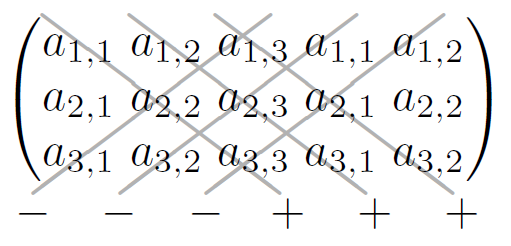
\includegraphics[width=7cm]{Sarrus-Regel}
%            \caption{Sarrus-Regel}
            \label{fig:sarrus}
        \end{figure}
        \end{Def}
        
        
        \subsubsection{Entwicklungssätze}
        \begin{Def}
            Sei $a_{ij}$ der j-te Eintrag in der i-ten Zeile.
            \begin{itemize}
                \item $\sum_{i = 1}^{n} (-1)^{i + j} \cdot a_{ij} \cdot det(A_{i,j})$ Entwicklung nach \linkToRef[Zeilenvektor]{Spalte} $i$
                \item $\sum_{j = 1}^{n} (-1)^{i + j} \cdot a_{ij} \cdot det(A_{i,j})$ Entwicklung nach \linkToRef[Zeilenvektor]{Zeile} $j$
            \end{itemize}
        \end{Def}
    
\newpage
\section{Eigenwerte}
\label{Eigenwert}
\begin{Def}
Ein Eigenvektor einer Abbildung ist in der linearen Algebra ein vom Nullvektor verschiedener Vektor, dessen Richtung durch die Abbildung nicht verändert wird. Ein Eigenvektor wird also nur skaliert und man bezeichnet den Skalierungsfaktor als Eigenwert der Abbildung.
\end{Def}

\begin{Def}[Eigenwerte und Eigenvektoren]
\label{Eigenvektor}
Sei $A \in \mathbb{K}^{n \times n} $, dann heißt $\lambda \in \mathbb{K} $ Eigenwert, falls ein Vektor $v \in \mathbb{K}^{n} \setminus \{0\} $ existiert, mit $A \cdot v = \lambda \cdot v$. $v$ heißt dann \textbf{Eigenvektor} zum Eigenwert $\lambda$\\

$A \cdot v = \lambda \cdot v \Leftrightarrow (A - \lambda \cdot Id) \cdot v = 0$ \\

\end{Def}

\begin{Notiz}
Eigenwerte charakterisieren wesentliche Eigenschaften linearer Abbildungen, etwa ob ein entsprechendes lineares Gleichungssystem eindeutig lösbar ist oder nicht.
\end{Notiz}

\subsection{Charakteristisches Polynom}
\begin{Def}
$X_A(\lambda) := det(A - \lambda \cdot Id)$
\end{Def}

\begin{Satz}
Nullstellen von $X_A$ sind Eigenwerte von $A$.
\end{Satz}

\begin{Def}[algebraische Vielfacheit]
    $m_a(\lambda)$ ist die Vielfacheit der Nullstelle $\lambda$ im charakteristischen Polynom $X_A$.
\end{Def}

\begin{Def}[geometrische Vielfacheit]
    \begin{align*}
        m_g(\lambda) := dim(E_\lambda)
    \end{align*}
\end{Def}
        TODO def: Eigenraum

\newpage
\section{Komplexe Zahlen}

\begin{Def}
    \begin{align*}
    \mathbb{C} :&= \left\{ \begin{pmatrix} a & b \\ -b & a \end{pmatrix} \middle| a,b \in \mathbb{R} \right\} \\
    &= \{ a \cdot I_2 + b \cdot i |a,b \in \mathbb{R} \}
    \end{align*}
    mit $i := \begin{pmatrix} 0 & 1 \\ -1 & 0 \end{pmatrix}$
\end{Def}

\begin{Def}
\begin{align*}
\mathbb{C} &= \{ a + bi | a,b \in \mathbb{R} \}\\
i^2 &= -1
\end{align*}
\end{Def}

\subsection{Real- und Imaginärteil}

\begin{Def}[Realteil]
    \begin{align*}
        a = Re(z)
    \end{align*}
\end{Def}

\begin{Def}[Imaginärteil]
    \begin{align*}
        b = Im(z)
    \end{align*}
\end{Def}

\newpage
\section{Die Google-Matrix und stochastische Matrizen}

\begin{Def}
Die Spaltensummen einer Matrix sind 1.
\end{Def}

\newpage
\section{Skalarprodukt}

\begin{Def}
    Für $v = \begin{pmatrix} x_1 \\ \vdots \\ x_n \end{pmatrix}$ und $w = \begin{pmatrix} y_1 \\ \vdots \\ y_n \end{pmatrix} \in K^n$ ist das Skalarprodukt:
    \begin{align*}
        \left< v, w \right> := \sum_{i=1}^n x_i y_i (= v^T w) \in K
    \end{align*}
\end{Def}

\begin{Notiz}
    Zeilenweise multiplizieren und die Teil Ergebnisse addieren.\\
    Aus der Schule bekanntes Verfahren: "`Kringel Operator'': $\circ$
    \begin{align*}
        \begin{pmatrix}
            a_1 \\ a_2 \\ a_3
        \end{pmatrix}
        \circ
        \begin{pmatrix}
            b_1 \\ b_2 \\ b_3
        \end{pmatrix} = a_1b_1 + a_2b_2 + a_3b_3
    \end{align*}
\end{Notiz}

\begin{Warnung}
    Die Notation $\left< v,w \right>$ ist leicht zu verwechseln mit dem Spann!
\end{Warnung}

\newpage
\section{Symmetrische Matrizen}

\begin{Def}
Eine Matrix ist symetris, falls gilt:
\begin{align*}
A = A^T
\end{align*}
\end{Def}

\newpage
\section{Anwendungen in der Graphentheorie}

\begin{Def}
    \begin{align*}
        G = (V, E)
    \end{align*}
    Wobei $V$ die Menge der Knoten (engl. \textit{vertices}) darstellt, und $E$ die Menge der Kanten (engl. \textit{edges})
\end{Def}

\begin{Def}[Adjazenzmatrix]
    Die Adjazenzmatrix gibt die Kanten zwischen den Knoten an.
\end{Def}

\newpage
\section{Rezepte}
\label{Rezepte}

\subsection{Lösen eines LGS}

\begin{enumerate}
\item \linkTo{LGS} in eine \linkTo{Matrix} schreiben
\item \linkToRef[Gauss]{Gauß-Algorithmus} anwenden, um strenge \linkTo{Zeilenstufenform} zu erhalten
\item 
    \begin{enumerate}
        \item direkt alle Elemente ablesen, falls möglich
        \item 
            \begin{itemize}
            \item Gleichung aufstellen ($n-rg(A) > \#$ freier Variablen)
            \item Aus Gleichungen Lösungsmenge bilden (als Vektoren)
            \item Lösungsmenge als Spann schreiben
            \end{itemize}
    \end{enumerate}
\end{enumerate}

\subsection{Lösbarkeit von LGS}

Bringe die \linkTo{erweiterete Koeffizentenmatrix} in \linkTo{Zeilenstufenform}. 

Es wird keine \textbf{strenge} \linkTo{Zeilenstufenform} benötigt.

Lösbar, wenn gilt \linkToRef[Rang]{$rg(A|B) = rg(A)$}.

Weitere Unterscheidung:
\begin{itemize}
\item Lösung eindeutig, wenn $ rg(A|b) = rg(A) = n$
\item Lösung \textbf{nicht} eindeutig, wenn $rg(A) < n$ (und $n - rg(A) = $ Anzahl freier Variablen)
\end{itemize}

\subsection{Untervektorraum}

\begin{enumerate}
\item Wenn es sich um die Lösungsmenge eines \linkToRef[homogenes LGS]{homogenen LGS} (also  $\{x|Ax=0\}$ handelt ist es ein \linkTo{Untervektorraum}
\item Unter(vektorraum)kriterien prüfen: 
        \begin{enumerate}[label={(\arabic*)}]
		\item % (1)
		nicht leer, insbesondere muss 0 enthalten sein: $U \neq \emptyset ~~|~~ 0 \in V$ 
		
		\item % (2)
		Addition abgeschlossen: $\forall v,w \in U \Rightarrow v + w \in U$ 
		
		\item % (3)
		Multiplikation abgeschlossen: $\forall a \in K, v \in U \Rightarrow a \cdot v \in U$
	\end{enumerate}
\end{enumerate}

\begin{Notiz}
$U \subseteq V-UVR \Leftrightarrow U$ mit Verknüpfung $+,\cdot$ selbst VR.
\end{Notiz}



\begin{Beispiel}
\begin{itemize}
\item % b)
		$M_2 = \{x \in \mathbb{R}^n | x_1 \geq 0\}$
		\begin{enumerate}[label={(\arabic*)}]
			\item % (1)
			$O_n \in M_2 \Rightarrow M_2 \neq \emptyset \checkmark$
			
			\item % (2)
			Sei $x,y \in M_2 \Rightarrow x_1 \geq 0, y_1 \geq 0 \Rightarrow z = x + y = (x_1 + y_1, ..., x_n + y_n) \Rightarrow z \in M_2 \checkmark$
			
			\item % (3)
			$u = (1, 0, ..., 0) \in M_2$, aber $(-1) \cdot u = (-1, 0, ..., 0) \notin M_2$ \\
			$M_2$ ist kein UVR.
		\end{enumerate}
		
		\item % c)
		$M_3 = \{x \in \mathbb{R} | x_1 - 2x_2 = 0\}$
		\begin{enumerate}[label={(\arabic*)}]
			\item % (1)
			$O_n \in M_3 \Rightarrow M_3 \neq \emptyset \checkmark$
			
			\item % (2)
			$x,y \in M_3 \Rightarrow x_1 - 2x_2 = 0 = y_1 - 2y_y \Rightarrow (x_1 + y_1) - 2(x_2 + y_2) = 0 \Rightarrow x + y \in M_2 \Rightarrow z = x + y = (x_1 + y_1, ..., x_1 + y_y) \in M_3 \Leftrightarrow x_1 + y_1 - 2(x_2 + y_2) = 0 \Leftrightarrow x_1 - 2x_2 + y_1 - 2y_2 = 0 \Leftrightarrow x,y \in M_3$
			
			\item % (3)a
			$a \in \mathbb{R}, x \in M_3$ (also $x_1 - 2x_2 = 0$) $\Rightarrow ax = (ax_1, ax_2, ..., ax_y) \in M_3 \Leftrightarrow ax_1 - 2ax_2 = 0 \Leftrightarrow a(x_1 - 2x_2) = 0 \Leftrightarrow x \in M_3 \Rightarrow M_3$ ist UVR
		\end{enumerate}
\end{itemize}
\end{Beispiel}

\subsection{Basis eines Spanns von Vektoren}

\begin{enumerate}
\item Schreibe alle Vektoren \underline{liegend} übereinander
\item \linkToRef[Gauss]{Gauß} anwenden, um \linkTo{Zeilenstufenform} zu erhalten
\item Die von 0 verschiedenen Zeilen bilden stehend geschrieben die Basisvektoren
\end{enumerate}

\subsection{Basen}

\begin{itemize}
\item $S$ Basis von $V \Leftrightarrow dim(V) = n$ und $S$ linear unabhängig  $ dim(V) = n = |S|$
\item $n < dim(V) \Rightarrow S $ kein EZS von $V$
\item $dim (V) < n \Rightarrow S $ linear abhängig
\end{itemize}

\begin{Beispiel}
\begin{itemize}
    \item % b)
		$V= \mathbb{R} [X] = \{a_0 + a_1x + a_2x^2 | a_0, a_1, a_2 \in \mathbb{R}\} $\\
		VL: $dim(V) = 3 \leq 2$ und $ S_0 = \{ 1, x, x^2\}$ ist eine Basis von $V$\\
		Ist $ S_1 = \{ 1, x + 1, x^2 + x + 1\}$ linear unabhängig | EZS | Basis?
		\begin{enumerate}[label={(\arabic*)}]
			\item % (1)
			zz. $\lambda_1 = \lambda_2 =  \lambda_3 = 0$\\
			$S_1$ ist linear abhängig: Seien $\lambda_1, \lambda_2, \lambda_3 \in \mathbb{R}$ mit $\lambda_1 \cdot 1 + \lambda_2 \cdot (x+1) + \lambda_3 \cdot (x^2 + x + 1) = 0 \Leftrightarrow (\lambda_1 + \lambda_2 +  \lambda_3) \cdot 1 + ( \lambda_2 +  \lambda_3) \cdot x + \lambda3x^2 = 0 $\\
			Da $1,x,x^2$ linear unabhängig $\Rightarrow$ LGS $\lambda_1, \lambda_2, \lambda_3 = 0 $\\
			$ \lambda_2 + \lambda_3 = 0, \lambda_3 = 0 \Rightarrow \lambda_1 + \lambda_2 + \lambda_3 = 0 \checkmark$ 
			
			\item % (2)
			Zeige, dass $S_1$ EZS von V ist. Es genügt zu zeigen, dass $S_0=\{1,x,x^2\} ~~\leq <S_1>$, da dann gilt:
			
			\[V = ~~ <S_0> ~~ = ~~ <1, x,x^2> ~~ \leq ~~ <S_1> ~~ \leq V ~~ \Rightarrow ~~ V = <S_1>\]
			
			\begin{itemize}
			\item $ 1 \in ~~ < 1, x + 1, x^2 + x + 1> ~~$, denn $1 = 1 \cdot 1 + 0 \cdot (x+1) + 0 \cdot (\dots)$ 
			\item $ x \in ~~ < 1, x + 1, x^2 + x + 1> ~~$, denn $x = -1 \cdot 1 + 1 \cdot (x+1)$ 
			\item $ x^2 \in ~~ < 1, x + 1, x^2 + x + 1> ~~$, denn $x^2 = 0 \cdot 1 - 1 \cdot (x+1) + 1 \cdot (x^2 + x + 1)$ 
			\end{itemize}
			Also gilt $S_1$ ist EZS.
			
			\item % (3)
			Nach Korollar 5.13:\\
			$dim(V) = 3 = |S_1| $ und $S_1$ ist EZS $\Rightarrow S_1$ ist Basis.
        \end{enumerate}
		
\end{itemize}

\end{Beispiel}

\subsection{Test auf lineare Unabhängigkeit}

\begin{enumerate}
\item Schreibe alle Vektoren \underline{stehend} nebeneinander
\item \linkToRef[Gauss]{Gauß} anwenden, um \linkTo{Zeilenstufenform} zu erhalten
\item 
    \begin{enumerate}
    \item Falls $rg(A) = \# $ der Spalten (also $n$) $\Rightarrow$ linear \textbf{unabhängig}
    \item Falls $rg(A) \neq n  \Rightarrow $ linear \textbf{abhängig} 
    \end{enumerate}
\end{enumerate}

\subsection{Lineare Codes}

\begin{enumerate}
\item ($G \rightarrow P$) $G = \begin{pmatrix} Id_g \\ \dots \\ A \end{pmatrix} \Rightarrow P = \begin{pmatrix} -A & \vdots & Id_p \end{pmatrix} $ 
\item ($P \rightarrow G$) Falls  $ P = \begin{pmatrix} -A & \vdots & Id_p \end{pmatrix} \Rightarrow G = \begin{pmatrix} Id_g \\ \dots \\ A \end{pmatrix}$ \\
$\rightarrow$ Falls nicht, löse das \linkTo{LGS} $P \cdot c = 0 $ und bestimme Basisvektoren $c_1, c_2, \dots, c_K$ des Lösungsraums $\Rightarrow G = (c_1~|~ c_2 ~|~ \dots ~|~ c_K)$
\end{enumerate}

\subsubsection{Informationen des Codes bestimmen}
    \begin{enumerate}
    \item Falls Generatormatrix gegeben:
        \begin{itemize}
        \item $G \in \mathbb{K}^{n \times k} \Rightarrow (n,k)$-Code
        \item d (Minimalabstand der Paritycheckmatrix)
            \begin{enumerate}
            \item Alle Wörter bilden und zählen\\
            oder
            \item Stelle Paritycheckmatrix auf und bestimme d
            \end{enumerate}
        \end{itemize}
    \item Falls Paritycheckmatrix gegeben:
        \begin{itemize}
        \item $P \in \mathbb{K}^{n~x~k} \Rightarrow k = n -rg(P) \Rightarrow (n,k)$-Code
        \item Bestimme d
        \end{itemize}
    \end{enumerate}


\subsubsection{Bestimmung des Minimalabstandes der Paritycheckmatrix}

\begin{tabular}{p{0.12\textwidth}p{0.85\textwidth}}
$d = 1$ & P hat \underline{eine} Nullspalte \\
$d = 2$ & P hat \underline{keine} Nullspalte, aber es gibt \underline{zwei} linear abhängige Spalten von P\\
$d = 3$ & P hat \underline{keine} Nullspalte, P hat  \underline{keine zwei} linear abhängige Spalten von P, aber P hat \underline{drei} Spalten von P, die linear abhängig sind\\
\end{tabular}

\subsubsection{Überprüfe ob das Codewort c geschickt wurde}
    \begin{enumerate}
    \item Berechne $ P \cdot c $\\
    Falls $ P \cdot c = 0 \Rightarrow $ wurde wahrscheinlich gesendet\\
    Falls $ P \cdot c \neq 0 \Rightarrow $ b) + c)
    \item Finde $f \in \mathbb{K}^n $ mit $P \cdot f = P \cdot c$, wobei f möglichst wenige Nicht-Nulleinträge haben soll\\
    $\Rightarrow$ Wie muss man das Codewort ändern, damit 0 rauskommt.
    $\Rightarrow$ 
    $\Rightarrow$ Starte mit den Standardvektoren $ = $ Spalten der Paritycheckmatrix\\
    $\Rightarrow$ dann vielfache der Standardvektoren\\
    $\Rightarrow$ dann Linearkombinationen des Spalten von P
    \item $\Rightarrow c' = c - f$ wurde wahrscheinlich gesendet
    \end{enumerate}

\subsubsection{Sonstige}

\begin{itemize}
\item Anzahl der Codewörter: $|\mathbb{K}|^k$
\item Informationsrate: $\frac{k}{n}$
\item Redundanz: n-k
\end{itemize}

\subsection{Lineare Abbildungen (1)} = Linearität

$\varphi : V \rightarrow W $ mit $V, W \mathbb{K}-VR$ heißt linear, falls
\begin{enumerate}
\item $\varphi (0_v) = 0_w $
\item $\forall  v, w \in V : f(v + w) = f(v) + f(w)$ (Additivität)
\item $\forall  v \in V, \forall  a \in \mathbb{K} : \varphi (a \cdot v) = a \cdot \varphi (v) $ (Homogenität)
\end{enumerate}

\begin{Beispiel}[Wichtiges Beispiel]

\[V = \mathbb{K}^n, W = \mathbb{K}^m, A \in \mathbb{K}^{m \times n}\]
$\Rightarrow \varphi_a : V \rightarrow W, x \mapsto A$

\end{Beispiel}

\subsection{Matrix invertieren}
Gegeben ist Matrix $A \in \mathbb{K}^{n~x~n}$\\
Berechne mit Gauß:\\
$\begin{pmatrix} A & \vdots & Id \end{pmatrix} \leadsto \begin{pmatrix} \textbf{\underline{Id}} & \vdots & A^{-1} \end{pmatrix} $\\
Falls dort \underline{nicht} die Identität steht, war / ist A nicht invertierbar da $ rg(A) \neq n $\\
$\Rightarrow A^{-1} $ ist die \textbf{Inverse}
\begin{Notiz}
Prüfe (immer), ob $A \cdot A^{-1} = Id$
\end{Notiz}

\begin{Notiz}
    Eine Matrix ist invertierbar, wenn $det(A) \neq 0$.
\end{Notiz}
\begin{Notiz}[Umkehrabbildung]
    Das Inverse einer Matrix wird für die Umkehrabbildung verwendet:
    \begin{align*}
    \varphi_A^{-1} = \varphi_{A}
    \end{align*}
\end{Notiz}

\subsection{Lineare Abbildungen (2)}

$\varphi : V \rightarrow W linear$
\begin{Notiz}
$|V| = |\mathbb{K}|^{dimV}$
\end{Notiz}
\begin{enumerate}
\item Bild$(\varphi) := \varphi(V) ~~ \underset{UVR}{\subset} ~~ W$\\
Falls $\varphi = \varphi_A \Rightarrow $ Bild $(\varphi) = ~<$ Spalten von $A~>$
\item Kern$(\varphi) = \varphi^{-1} (0_w) ~ \subset ~ W$\\
Falls $\varphi = \varphi_A \Rightarrow $ Kern $(\varphi) = \{x \in V | A \cdot x = 0 \}$
\item Urbild $\varphi^{-1} (w)$\\
Falls $\varphi = \varphi_A \Rightarrow \varphi^{-1} = \{x \in V | A \cdot x = w \} = A^{-1} \cdot w$, letzter Schritt, falls A invertierbar.
\begin{Notiz}
bidirektional = isomorph $\Leftrightarrow$ regulär $\Leftrightarrow$ invertierbar\\
VR-Isomorphismus bildet Basen auf Basen ab.
\end{Notiz}
\item Injektivität / Surjektivität / Bijektivität\\
$\varphi : V \rightarrow W$
    \begin{enumerate}
    \item injektiv, falls aus $\varphi (v) = \varphi (w) $ folgt $ v = w ~~~~~~ (\varphi (v - w) = 0)$
    \item surjektiv, falls $\varphi (v) = w$
    \item bijektiv, falls injektiv und surjektiv\\
    \begin{Notiz}
    $\varphi $ ist injektiv $\Leftrightarrow dim (Kern) \ngeq 1$ \\ 
    $\varphi $ ist injektiv $\Leftrightarrow Kern(\varphi) = \{0\}$ \\
    $\varphi $ ist surjektiv $\Leftrightarrow dim (Bild(\varphi)) = dim(W) = rg(A)$, letzter Schritt gilt, falls $\varphi = \varphi_A$ 
    \end{Notiz}
    \end{enumerate}
    \item Dimensionssatz: \\
    $\varphi : V \rightarrow W$ linear\\
    $dim(V) = dim(Kern (\varphi)) + dim(Bild(\varphi)) ~~~~~~~ dim(V) < \infty$
\end{enumerate}

\subsection{Wann ist eine Menge eine Basis?}

Wenn die Menge linear unabhägig ist und ein \linkTo{Erzeugendensystem} ist.\\
Falls $|S| > dim(V) \Rightarrow $ linear abhängig, insbesondere \underline{nicht} linear unabhängig.\\
Falls $|S| < dim(V) \Rightarrow $ \underline{kein} EZS.\\
$\Rightarrow$ Basis ist nur möglich, wenn $|S| = dim(V)$.\\
$\rightarrow$ Prüfe immer, ob S linear unabhängig ist \underline{oder} ob S ein EZS ist. Falls ja, ist es auch ein EZS bzw. linear unabhängig ist und somit S eine Basis von V ist.

\subsection{Darstellungsmatrizen}

\begin{Def}
Sei $V$ ein $K$-VR und $B = \{b_1, \dots, b_n\}$ von $V$\\


$\varphi : V \mapsto V $ lineare Darstellungsmatrix\\


$D_B(\varphi) \in \mathbb{K}^{n~x~n} $ beschreibt $\varphi$ bezüglich $B$.

\end{Def}

Für $j = 1, ..., n $:

\begin{enumerate}
\item Wende $\varphi$ auf die Basisvektoren $b_j$ an.
\item Schreibe $\varphi(b_j) \in V$ als Linearkombination bezüglich $B$ auf.
\item Schreibe die Koeffizenten der Linearkombination in die j-te Spalte von $D_B(\varphi)$
\end{enumerate}



\subsection{Bilder von Darstellungsmatrizen}

\begin{itemize}
\item Sei $\varphi: V \rightarrow W$ linear mit $B := \{b_1, b_2, \dots, b_n\}$ Basis von V. $C := \{c_1, c_2, \dots, c_m\}$ Basis von W. $B, W$ sind VR. $i = 1, \dots, n$. $D_{B\lambda}(\varphi) = 0_{\mathbb{K}^{n~x~n}}$
\item Berechne $\varphi(b_i)$
\item Stelle $\varphi(b_i)$ als Linearkombination der Basisvektoren $c_1, \dots, c_m$ dar.\\
$\varphi(b_i) = a_1 \cdot c_1 + a_2 \cdot c_2 + \dots + a_m c_m$
\item Schreibe die Koeffizenten als stehenden Vektor in die i-te Spalte von $D_{B,C} (\varphi)$\\
$\Rightarrow D_{B,C} (\varphi)$ ist die Darstellungsmatrix von $\varphi$ zur Basis B und C.
\end{itemize}

\subsection{Vektor als Linearkombination bezüglich einer Basis} \label{Linearkombination}

Vektor $v = \begin{pmatrix} 3 \\ 1 \\ 0\\ 1 \end{pmatrix} \in \mathbb{R}^4$ soll als Linearkombination bezüglich der Basis $B$ geschrieben werden.

\begin{align*}
v_1 = \begin{pmatrix} 1 \\ 0 \\ 1\\ 0 \end{pmatrix}, ~~~ v_2 = \begin{pmatrix} 0 \\ 1 \\ 0\\ 1 \end{pmatrix}, ~~~ v_3 = \begin{pmatrix} 1 \\ -1 \\ 2\\ 1 \end{pmatrix}, ~~~ v_4 = \begin{pmatrix} -1 \\ 0 \\ 2\\ 0 \end{pmatrix} \in \mathbb{R}^4
\end{align*}
Basis $B = \{v_1, v_2, v_3, v_4\}$ von $\mathbb{R}^4$\\
\begin{enumerate}
\item Erweiterte Matrix aufstellen mit Vektoren der Basis als Spalten der Matrix ($=A$) und dem Vektor $v$ ($=b$)
\item \linkToRef[Gauss]{Gauß-Algorithmus} ausführen und strenge Zeilenstufenform bilden
\item Linearkombination aus $b$ ablesen
\end{enumerate}


\begin{Beispiel}
\begin{align*}
\left(
\begin{array}{cccc|c}
1 & 0 & 1 & -1 & 3 \\
0 & 1 & -1 & 0 & 1\\
1 & 0 & 2 & 2 & 0\\
0 & 1 & 1 & 0 & 1
\end{array}
\right)
\Rightarrow
\left(
\begin{array}{cccc|c}
1 & 0 & 0 & 0 & 2 \\
0 & 1 & 0 & 0 & 1\\
0 & 0 & 1 & 0 & 0\\
0 & 0 & 0 & 1 & -1
\end{array}
\right)
\end{align*}
\end{Beispiel}


\subsection{Basistausch (zu linear unabhängig)}

Ist $v$ eine Linearkombination aus dem Basisvektor $v_i$ mit $ i \in I \subset \{1, \dots, n\}$, dann ist $B_i := B \setminus \{v_i\} \cup \{v\} $ mit $i \in I$ eine Basis von $V$, da für $i \notin I~~~ B_i$ linear abhängig ist. Für $i \in I$ ist $B_i$ ein EZS von $V_i$, da wie in jeder Linearkombination eines Vektors $v \in V$ den Basisvektor $v_i$ durch die anderen Basisvektoren $v_j $ mit $j \in I \setminus \{i\}$ und $v$ ersetzen können.


\begin{Notiz}
Wann ist $B_i := B \setminus \{v_i\} \cup \{v\} $ eine Basis?

Genau dann, wenn $v_i$ mit Koeffizenten $\neq 0$ in $v$ auftaucht.
\end{Notiz}

\begin{Beispiel}
Gegeben sei die Basis $B = \{v_1, v_2, v_3, v_4\}$ aus $\mathbb{R}^4$ und die Linearkombination $v = 2v_1 + 1v_2 - v_4$ bezüglich der Basis $B$.



Wir können genau diejenigen $v_i$’s, die in der Linearkombination von $v$ bezüglich der Basis
$B$ mit Koeffizient ungleich Null auftauchen durch $v$ ersetzen, so dass $B_i$ weiterhin eine Basis
ist. Dies geht also für $i = 1,2,4$

\begin{enumerate}
\item $v_1 = \frac{1}{2}v - \frac{1}{2}v_2 + \frac{1}{2} v_4$\\
    $i=1~~~~v_1, v_2, v_3, v_4 \in <~B_1~> = <~ \frac{1}{2}v - \frac{1}{2} + \frac{1}{2} v_4, v_2, v_3, v_4 ~>$
    
    
    $\Rightarrow B_1$ ist EZS der Länge $4 = dim(V)$ von $V$, also ist $B_1$ eine Basis
\item $v_2 = v - 2v_1 + v_4$\\
    $i=2~~~~v_1, v_2, v_3, v_4 \in \left< B_2 \right> = \left< v_1, v - 2v_1 + v_4, v_3, v_4 \right>$
    
    
    $\Rightarrow B_2$ ist EZS der Länge $4 = dim(V)$ von $V$, also ist $B_2$ eine Basis
\item $i=3~~~~v_3 \notin \left< B_3 \right> = \left< v_1, v_2, v_3, v_4 \right>$


    $\Rightarrow B_3$ ist kein EZS von $V$, also auch keine Basis
\item $v_4 = -v + 2v_1 + v_2$\\
    $i=4~~~~v_1, v_2, v_3, v_4 \in \left< B_4 \right> = \left< v_1, v_2, v_3, -v + 2v_1 + v_2 \right>$
    
    
    $\Rightarrow B_4$ ist EZS der Länge $4 = dim(V)$ von $V$, also ist $B_4$ eine Basis
\end{enumerate}
\end{Beispiel}

\subsection{Bestimmung von Bild, Kern von $\varphi$ und Urbild von $u$}

\begin{Def}
Sei $\varphi : V \rightarrow W $ eine Abbildung.
\begin{itemize}
\item Urbild von $B \subset W $ unter $\varphi$:
\[\varphi^{-1}(B) :=  \{v \in V | \varphi(v) = B\}\]
\item Bild von $A \subset W $ unter $\varphi$:
\[\varphi(A) :=  \{\varphi(v) | v \in A\}\]
\item Kern von $\varphi$:
\[Kern(\varphi) = \varphi^{-1}(\{0_w\})\]
\item Bild von $\varphi$:
\[Bild(\varphi) = \varphi(V)\]
\end{itemize}
Falls $\varphi$ linear ist:

\begin{itemize}
\item Kern $\varphi$ ist UVR von $V$
\item Bild $\varphi$ ist UVR von $W$
\item $\varphi$ ist injektiv $\Leftrightarrow$ Kern $\varphi = \{0_v\}$, oder dim Kern $\varphi \neq 0$ 
\item $\varphi$ ist surjektiv $\Leftrightarrow$ Bild $\varphi = W$, oder dim Bild $\varphi =$ dim W 
\end{itemize}

Es gilt der Dimensionssatz:
\[dim(V) = dim(Kern~~\varphi) + dim(Bild~~\varphi)\]

\end{Def}

Sei $B=\{b_1, \dots, b_n\}$ Basis von $V_j ~~~ C:= \{c_1, \dots, c_m\}$ Basis von $W$.
\begin{enumerate}
\item Bestimme die Darstellungsmatrix $D_{B,C} (\varphi) : $ siehe oben
\item Bestimme den Kern und das Bild der Matrix $D_{B,C}(\varphi)$
    \begin{itemize}
    \item Kern $D_{B,C}(\varphi) = \left< v_1, \dots, v_p \right>$
    \item Bild $B_{B,C}(\varphi) = \left< w_1, \dots, w_q \right>$
    \item Urbild: Löse 
    \[U := \{x \in \mathbb{K}^n | D_{B,C}(\varphi) \cdot x = (u) c ??????\} = U = \{v + a_1v_1 + \dots + a_ov_o | a_i \in \mathbb{K}\}\]
    \item 
    \begin{itemize}
    \item Kern $\varphi = \left< (v_1)_B, (v_2)_B, \dots, (v_p)_B \right> = \left<v_1, v_2, \dots, v_p \right>$
    \begin{Notiz}
    $ = $ sei definiert als "`Übersetze die Basisdarstellung zurück in die natürliche Darstellung von $V_i$ "'

    (z.B. von Vektor $\rightarrow$ Matrix, von Vektor $\rightarrow$ Polynom,von Vektor $\rightarrow$ Funktion)
    \end{Notiz}
    \item Bild $\varphi = \left< (w_1)_c, (w_2)_c, \dots, (w_q)_c \right>\overset{zurueckuebersetzen}{=} \left<w_1, w-2, \dots, w_q \right>$
    \item Urbild $\varphi^{-1}(v) = \{(v)_B + a_1 \cdot (v_1)_B + \dots + a_o(v_o)_B \} \overset{zurueckuebersetzen}{=} \{v + a_1 \cdot v_1 + \dots + a_ov_o\}$
    \end{itemize}
    $\Rightarrow dim(Kern \varphi) = dim(Kern~~ D_{B,C}(\varphi))$
\end{itemize}
\end{enumerate}

\newpage
\subsection{Basiswechselmatrix $S_{C,B}$}

\begin{Def}
  "`Koordinaten in C"' $ = S_{C,B} \cdot $ "`Koordinaten in B"'
  \begin{align*}
  S_{C,B} &= D_{B,C}(id)\\
  &~ \\
  S_{B,C} &= S_{C,B}^{-1}
  \end{align*}
  \begin{Notiz}
  Bei der Basiswechselmatrix heißt $C,B$ dass zu C gewechselt wird. Bei der Darstellungsmatrix steht $B,C$ für das man die Aktion einer linearen Abbildung bezüglich der Basisdarstellung B betrachtet und was als Ergebnis in Basisdarstellung von $C$ dabei herauskommt
  \end{Notiz}
\end{Def}



\begin{Def}
  Sei $\varphi : V \rightarrow W $ linear und $B,B'$ sind Basen von $V,~~~ C, C'$ sind Basen von W
  \begin{align*}
  D_{B',C'}(\varphi) = S_{C', C} \cdot D_{B,C} (\varphi) \cdot S_{B,B'}
  \end{align*}
\end{Def}

\begin{Def}
  Sei $\varphi : V \rightarrow W $ linear und $B,B'$ sind Basen von $V$
  \begin{align*}
  D_{B'}(\varphi) = S_{B',B} \cdot D_B(\varphi) \cdot S_{B,B'} = S_{B,B'}^{-1} \cdot D_B(\varphi) \cdot S_{B,B'}
  \end{align*}
  \begin{Notiz}
  $D_{B'}$ steht für $D_{B', B'}$
  \end{Notiz}
\end{Def}

\begin{Def}
  Falls $E$ die Einheitsbasis ist, dann ist $S_{E,B}$ immer gleich $S_{E,B} = (b_1|b_2|\dots | b_n)$
\end{Def}

\textbf{Algorithmus für $S_{C,B}$:}
\[(c_1 | c_2| \dots | c_n || b_1 | b_2 | \dots | b_n) \overset{Gauss}{\rightsquigarrow} (Id | S_{C,B})\]
\textbf{Alternativ:}
\begin{enumerate}
\item Schreibe $b_j$ als Linearkombination von C
\item Schreibe die Koeffizenten in die j-te Spalte von $S_{C,B}, ~~j=1,..., n$
\end{enumerate}

\textbf{Algorithmus für $D_{B,C}$:}
\[(c_1 | c_2| \dots | c_n || \varphi(b_1) | \varphi(b_2) | \dots | \varphi(b_n)) \overset{Gauss}{\rightsquigarrow} (Id | D_{B,C}(\varphi))\]


\begin{Notiz}[Notiz zu Algorithmus]
\begin{itemize}
\item geht nur bei Vektoren
\item Polynome und Matrizen als Vektor schreiben (bzgl. Einheitsmatrix)
\end{itemize}
\end{Notiz}



\subsection{Determinanten}

\begin{Notiz}
  $A$ ist invertierbar $\Leftrightarrow rg(A) = n \Leftrightarrow det(A) \neq 0$
\end{Notiz}

Die Abbildung $det : \mathbb{K}^{n~x~m} \rightarrow \mathbb{K} $ ist wie folgt definiert: 
\begin{enumerate}
\item Falls $ A = 
\begin{pmatrix} 
a_1 &  &  & * \\
 & a_2 &  &  \\
 &  & \ddots &  \\
0 &  &  & a_n
\end{pmatrix} \Rightarrow det(A) = a_1 \cdot a_2 \cdot ... \cdot a_n$ 
\item Falls die Matrix $B$ sich aus $A$ ergibt, indem man zwei Zeilen oder Spalten vertauscht, dann ist $det(B) = - det(B)$.
\item Falls $B$ sich aus $A$ ergibt, indem man ein Vielfaches einer Zeile oder Spalte zu einer \underline{anderen} Zeile oder Spalte addiert, dann ist $det(A) = det(B)$.
\item Falls $B$ sich aus $A$ ergibt, indem man ein $\frac{1}{\lambda}$-faches einer Zeile oder Spalte bildet, dann ist $det(B) = \lambda \cdot det(A)$.
\end{enumerate}

\subsubsection{Berechne die Determinante von $A$}

Wende Gauß auf $A$ an unter Berücksichtigung von 2. - 4. bis Fall 1 eintritt.

\subsubsection{Rechenregeln}

Siehe \linkTo{Rechenregeln Determinanten}


Und siehe \linkTo{Sarrus-Regel}

\subsubsection{Entwicklung nach Zeilen der Spalten}

\begin{Notiz}
Schachbrettmuster: $
\begin{pmatrix}
+ & - & + & - \\
- & + & - & + \\
+ & - & + & - \\
- & + & - & +
\end{pmatrix}
$
\end{Notiz}

\begin{itemize}
\item Sei $A_{i,j}$ die Matrix, die sich aus $A$ ergibt, indem man die i-te Zeile und die j-te Spalte streicht.
\item Entwickle nach der i-ten Zeile:
\[det (A) = \sum_{j=1}^{n} (-1)^{i+j} \cdot a_{ij} \cdot det(A_{ij}) \]
\item Entwickle nach der j-ten Zeile:
\[det (A) = \sum_{i=1}^{n} (-1)^{i+j} \cdot a_{ij} \cdot det(A_{ij}) \]
\end{itemize}

\subsection{Eigenwerte und Eigenvektoren}


\subsection{Kern einer Abbildung}

Abbildung \(\varphi: x \rightarrow Ax\)
\begin{enumerate}[label={(\arabic*)}]
    \item Matrix $A$ mit \linkToRef[Gauss]{Gauß} auf Zeilenstufenform bringen
    \item $dim(Kern(A)) = rg(A)$
    \item Finde Vektoren die Multipliziert mit $A$ multipliziert 0 ergeben.
\end{enumerate}

\begin{Beispiel}
    \begin{align*}
        A &= \begin{pmatrix} 1 & 0 & 2 & 1 \\
2 & 1 & 0  & 1 \\
2 & 2 & -4 & 0
\end{pmatrix}\\
        \begin{pmatrix} 1 & 0 & 2 & 1 \\
        2 & 1 & 0  & 1 \\
        2 & 2 & -4 & 0
        \end{pmatrix} &\rightsquigarrow \begin{pmatrix} 1 & 0 & 2 & 1 \\
        0 & 1 & -4  & -1 \\
        0 & 0 & 0 & 0
        \end{pmatrix}\\
        Kern(A) &= \left\{ \begin{pmatrix} -2 \\ -4 \\ 1 \\ 0 \end{pmatrix}, \begin{pmatrix} -1 \\ 1 \\ 0 \\ 1 \end{pmatrix} \right\}
    \end{align*}
\end{Beispiel}

\section{Abkürzungen}

\begin{tabular}{p{0.12\textwidth}p{0.85\textwidth}}
\textbf{EZS} & \linkTo{Erzeugendensystem}\\
\textbf{LGS}\label{LGS} & \linkTo{Lineares Gleichungssystem} \\
\textbf{Spann} & \linkTo{Spann} / Lineare Hülle\\
\textbf{V~K$-$VR} & Sei $V$ ein $K$-\linkTo{Vektorraum}\\
\textbf{VR} & \linkTo{Vektorraum} \\
\end{tabular}

\section{Source-Code}

\href{https://github.com/ibhh/LinAlgZusammenfassung}{Github - LinAlgZusammenfassung - https://github.com/ibhh/LinAlgZusammenfassung}

\end{document}
